\documentclass[manuscript, letterpaper]{aastex6}

% to-do list
% ----------
% - zeroth draft
% - search for occurrences of HOGG, DWH, APW, DFM, HWR in the text to make sure all issues are addressed.

% style notes
% -----------
% - This file generates by Makefile; don't be typing ``pdflatex'' or some bullshit.
% - Line break between sentences to make the git diffs readable.
% - Simple Monte Carlo gets a capital S to indicate that it is a defined thing.
% - Use \, as a multiply operator.
% - Reserve () for function arguments; use [] or {} for outer shit.
% - Always prior pdf or posterior pdf, never prior or posterior (that's your arse).
% - Use \sectionname not Section, \figname not Figure, \documentname not Article or Paper or paper.

\include{gitstuff}
% ----------------------------------- %
% start of AASTeX mods by DWH and DFM %
% ----------------------------------- %

\setlength{\voffset}{0in}
\setlength{\hoffset}{0in}
\setlength{\textwidth}{6in}
\setlength{\textheight}{9in}
\setlength{\headheight}{0ex}
\setlength{\headsep}{\baselinestretch\baselineskip} % this is 2 lines in ``manuscript''
\setlength{\footnotesep}{0in}
\setlength{\topmargin}{-\headsep}
\setlength{\oddsidemargin}{0.25in}
\setlength{\evensidemargin}{0.25in}

\linespread{0.54} % close to 10/13 spacing in ``manuscript''
\setlength{\parindent}{0.54\baselineskip}
\hypersetup{colorlinks = false}
\makeatletter % you know you are living your life wrong when you need to do this
\long\def\frontmatter@title@above{
\vspace*{-\headsep}\vspace*{\headheight}
\noindent\footnotesize
{\noindent\footnotesize\textsc{\@journalinfo}}\par
{\noindent\scriptsize Preprint typeset using \LaTeX\ style AASTeX6\\
With modifications by David W. Hogg and Daniel Foreman-Mackey
}\par\vspace*{-\baselineskip}\vspace*{0.625in}
}%
\makeatother

% Section spacing:
\makeatletter
\let\origsection\section
\renewcommand\section{\@ifstar{\starsection}{\nostarsection}}
\newcommand\nostarsection[1]{\sectionprelude\origsection{#1}}
\newcommand\starsection[1]{\sectionprelude\origsection*{#1}}
\newcommand\sectionprelude{\vspace{1em}}
\let\origsubsection\subsection
\renewcommand\subsection{\@ifstar{\starsubsection}{\nostarsubsection}}
\newcommand\nostarsubsection[1]{\subsectionprelude\origsubsection{#1}}
\newcommand\starsubsection[1]{\subsectionprelude\origsubsection*{#1}}
\newcommand\subsectionprelude{\vspace{1em}}
\makeatother

\widowpenalty=10000
\clubpenalty=10000

\sloppy\sloppypar

% ------------------ %
% end of AASTeX mods %
% ------------------ %


% packages
\definecolor{cbblue}{HTML}{3182bd}
\usepackage{microtype}  % ALWAYS!
\usepackage{amsmath}
\hypersetup{backref,breaklinks,colorlinks,urlcolor=cbblue,linkcolor=cbblue,citecolor=black}

% define macros for text
\newcommand{\project}[1]{\textsl{#1}}
\newcommand{\acronym}[1]{{\small{#1}}}
\newcommand{\apogee}{\project{\acronym{APOGEE}}}
\newcommand{\sdssiii}{\project{\acronym{SDSS-III}}}
\newcommand{\samplername}{\project{The~Joker}}
\newcommand{\emcee}{\project{emcee}}
\newcommand{\dr}{\acronym{DR13}}
\newcommand{\documentname}{\textsl{Article}}
\newcommand{\sectionname}{Section}
\newcommand{\figname}{Figure}

% define macros for math
\newcommand{\meterspersecond}{\mathrm{m\,s^{-1}}}
\newcommand{\asini}{\ensuremath{a_1\,\sin i}}
\newcommand{\given}{\,|\,}
\newcommand{\dd}{\mathrm{d}}
\newcommand{\transpose}[1]{{#1}^{\mathsf{T}}}
\newcommand{\inv}[1]{{#1}^{-1}}
\newcommand{\msun}{\mathrm{M}_\odot}
\newcommand{\rsun}{\mathrm{R}_\odot}
\newcommand{\kms}{\mathrm{km}~\mathrm{s}^{-1}}
\newcommand{\bs}[1]{\boldsymbol{#1}}

% TODO
\newcommand{\todo}[1]{{\color{red}TODO: #1}}

\begin{document}\sloppy\sloppypar\raggedbottom\frenchspacing % trust me

\title{\samplername: A custom Monte Carlo sampler \\
  for binary-star and exoplanet radial velocity data}
\author{Adrian~M.~Price-Whelan\altaffilmark{\pu,\adrn},
        David~W.~Hogg\altaffilmark{\ccpp,\mpia},
        Daniel~Foreman-Mackey\altaffilmark{\uw,\sagan},
        Hans-Walter~Rix\altaffilmark{\mpia}
}

% Affiliations
\newcommand{\pu}{1}
\newcommand{\adrn}{2}
\newcommand{\ccpp}{3}
\newcommand{\mpia}{4}
\newcommand{\uw}{5}
\newcommand{\sagan}{6}

\altaffiltext{\pu}{Department of Astrophysical Sciences,
                   Princeton University, Princeton, NJ 08544, USA}
\altaffiltext{\adrn}{To whom correspondence should be addressed:
                     \texttt{adrn@princeton.edu}}
\altaffiltext{\ccpp}{Center for Cosmology and Particle Physics,
                     Department of Physics,
                     New York University, 4 Washington Place,
                     New York, NY 10003, USA}
\altaffiltext{\mpia}{Max-Planck-Institut f\"ur Astronomie,
                     K\"onigstuhl 17, D-69117 Heidelberg, Germany}
\altaffiltext{\uw}{Astronomy Department, University of Washington,
                   Seattle, WA 98195, USA}
\altaffiltext{\sagan}{Sagan Fellow}

\begin{abstract}
% Context
Given sparse or low-quality radial-velocity measurements of a star, there are
often many qualitatively different stellar or exoplanet companion orbit models
that are consistent with the data.
The consequent multimodality of the likelihood function leads to extremely
challenging search, optimization, and MCMC posterior sampling in the space of
orbital parameters.
% Aims
Here we create a custom-built Monte Carlo sampler that can produce a posterior
sampling for orbital parameters given any number of noisy radial-velocity
measurements~--~even when the likelihood function is poorly behaved.
% Methods
The six standard orbital parameters can be split into the four non-linear
parameters (period, eccentricity, argument of pericenter, phase) and two linear
parameters (velocity amplitude and barycenter velocity).
We capitalize on this separability and build a variant of Simple Monte Carlo
sampling, in which we densely sample the non-linear orbital parameters, and
perform rejection sampling using a marginalized likelihood, marginalizing out
the linear orbital parameters.
In the case of sparse or uninformative data, the sampling obtained by the Simple
Monte Carlo is generally multimodal and dense.
With informative data, the sampling is generally unimodal but insufficient.
In the unimodal case, we follow the Simple Monte Carlo with standard MCMC to
make the sampling more substantial.
% Results
The method produces correct samplings in orbital parameters for data sets
that include as few as three noisy time points.
\samplername\ can therefore be used to (1) verify that the likelihood function
is unimodal \todo{(None of the datasets will actually have unimodal
likelihoods\ldots what does this mean?)} for a given set of data, and (2)
produce proper samplings of multimodal pdf to use in hierarchical modeling
(e.g., population modeling).
We give some examples that show how the posterior probability depends extremely
strongly on the number and time coverage of the observations and their
uncertainties.
\end{abstract}

\keywords{
  binaries: spectroscopic
  ---
  methods: data analysis
  ---
  methods: statistical
  ---
  planets and satellites: fundamental parameters
  ---
  surveys
  ---
  techniques: radial velocities
}

\section{Introduction} \label{sec:intro}

\todo{DFM, HWR: This section needs work, and references! Any suggestions would
be great.}
Precise radial-velocity measurements of stars have transformed
astrophysics in the last decades:
They have permitted the discovery of the first planets around other stars,
including especially the unanticipated but common ``hot Jupiters,''
and have been used to discover or confirm hundreds
of planets.
Radial velocity measurements have also been used to find substellar,
degenerate, and black-hole companions to more normal stars, and hold
the promise of delivering the full population statistics for binary
(and trinary) star systems.

With many new stellar spectroscopic surveys operating or under
construction, we expect to have good quality spectra for millions
of stars in the next few years.
Most of these surveys have at least some targets---and many have many
targets---that are observed multiple times.
These surveys can (as an auxilliary or primary goal of their observing
strategies) generate discoveries of planetary, substellar, and stellar
companions.
These discoveries, in turn, will feed population inferences, follow-up
programs, and projects to refine precise stellar models.

However, when radial-velocity observations are not designed with
unambiguous detection and discovery in mind, usually there are
multiple possible binary-star models that are consistent with any
small number of radial-velocity measurements that show stellar
acceleration.
That is, a small number of radial velocity measurements~--~even when the
uncertainties are small~--~will lead to posterior beliefs about companion
orbits and masses that put substantial plausibility onto multiple
qualitatively different solutions.
In other words, modest numbers of radial-velocity measurements create a
likelihood function that is highly multi-modal in the relevant parameter spaces
(e.g., Keplerian orbital parameters).
There are currently no methods known for exploring these highly multimodal
functions and delivering correct posterior samplings and reliable
probabilistic statements about detection and characterization.
\todo{Why are we not happy with nested sampling?}

Here we make an attempt at correcting this problem.
Our approach is to build custom posterior sampling methods that capitalize on
the structure of the binary-star (or star--exoplanet) kinematics to generate
robust samplings with only modest computational cost.
In what follows, we use the term ``binary'' for any system with an observed
source (the primary, e.g., a star), whose radial velocity variations are
explained through gravitational two-body interactions with another object (the
companion, e.g., star, exoplanet, stellar remnant).

The structure of this \documentname\ is as follows:
We state our assumptions, and demonstrate that we have a
method that is correct under those assumptions.
\todo{HOGG: I know that you like this ``provably correct'' terminology but I
(DFM) really think it doesn't add anything to the discussion.}
We perform experiments with the method to understand its properties and
limitations.
We finish by discussing the astrophysical applicability and potential of the
method, and the changes we would have to make if we weakened our assumptions, or
if we don't weaken our assumptions but they indeed prove to be far from correct.

\section{Assumptions and method} \label{sec:method}

\todo{This section also needs work, and references}

In order to set up a well-posed problem and build a path to a
definite solution, we make a set of non-trivial assumptions about the
stellar systems we will use and observations thereof.
\begin{itemize}\itemsep0ex  % <- #yourefired
\item We assume that we have measurements of the radial velocity of a
  star, and that the time dependence of the expectation of that radial
  velocity is well described by the gravitational orbit of a pair of
  point masses (the two-body problem). We assume that the times are
  (effectively) perfectly known, and in an inertial frame (for
  example, Solar-System barycenter Julian date).
  Here we only consider the case of a single-line spectroscopic binary system,
  where we do not have measurements of the companion's orbit.
\item We assume that each star has exactly one companion, and that the
  radial-velocity measurements are not contaminated by nor affected by
  any other bodies. Since we permit the effective mass of the
  exactly-one companion to go to zero, this assumption is really that
  the star has zero or one companion.
\item We assume that the noise contributions to individual
  radial-velocity measurements are well described as draws from
  zero-mean normal (Gaussian) distributions with correctly known
  variances. We assume that there are no outliers.
\item In addition to all these, we put particular, fairly sensible
  prior probability density functions on all the orbital parameters,
  described below.
\end{itemize}
Each of these assumptions can be challenged: in particular we expect some stars
to have additional companions, and we expect there to be outliers and
unaccounted sources of noise.
We will return to these assumptions, and the consequences of relaxing them, in
\sectionname~\ref{sec:discussion}.

In the two-body celestial mechanics problem (\citealt{Kepler:1609}; and here we
are working in a parameterization similar to that of \citealt{Murray:2010}), and
under our above-stated assumptions, the radial-velocity expectation can be
parameterized by six parameters, which we choose to be period $P$, projected
semi-major axis of the primary $\asini$, a phase $\phi_0$ corresponding to a
time of pericenter passage,\footnote{In our implementation, we subtract off the
median time from our data before starting so this phase actually corresponds to
the time of pericenter passage relative to the median time.} the eccentricity
$e$, an argument of perihelion $\omega$, and a constant system barycenter radial
velocity $v_0$.
The radial velocity $v$ at time $t$ is then given by (see also
equation~63 in \citealt{Murray:2010})
\begin{equation}
  v(t;\bs{\theta}) = v_0 + K\,[\cos(\omega + f) + e\,\cos\omega]
\end{equation}
where the $\bs{\theta}$ represents the free parameters, $K$ is the velocity
semi-amplitude, $f$ is the true anomaly given by
\begin{align}
  K &= \frac{2\pi\,\asini}{P\,\sqrt{1-e^2}}\\
  \cos f &= \frac{\cos E - e}{1 - e\, \cos E}
\end{align}
and the eccentric anomaly, $E$, must be solved for with the mean
anomaly, $M$,
\begin{align}
  M &= \frac{2\pi\, t}{P} - \phi_0\\
  M &= E - e\,\sin E \quad .
\end{align}
Of these parameters, four ($P$, $\phi_0$, $e$, $\omega$) are
non-linearly related to the radial-velocity expectation, and two
($\asini$, $v_0$) are linearly related.

Fundamentally, our method is to perform \emph{Simple Monte Carlo} in
the non-linear parameters, and analytically marginalize over the linear
parameters.
The method capitalizes on the following aspects of the problem
structure:
\begin{itemize}\itemsep0ex
\item There are both linear and non-linear parameters, and we can
  treat them differently; in particular, it is possible to
  analytically marginalize the linear parameters (provided that the
  noise model is well-behaved and the prior probability is conjugate).
\item There is a finite, time-sampling-imposed minimum size or
  resolution---in the period---of any features in the
  likelihood function. That is, there cannot be arbitrarily narrow
  modes in the multimodal posterior pdf.
\end{itemize}

Simple Monte Carlo is a method in which the prior probability density function
(prior pdf) is densely sampled, and then many of the samples are rejected by a
rejection-sampling step that uses the likelihood as the rejection scalar.
The rejection step works as follows:
\begin{enumerate}\itemsep0ex
\item For each sample $j$ in the prior pdf sampling of the four non-linear
  parameters, there is a (linear, not logarithmic) likelihood value $L_j$ (a
  probability for the data given the parameters).
\item There is a maximum value $L_{\rm max}$ that is the largest value of
  $L_j$ found across all of the samples in the prior sampling.
\item For each sample $j$, choose a random number $r_j$ between 0 and
  $L_{\rm max}$
\item Reject the sample $j$ if $L_j < r_j$.
\item The number of samples that survive the rejection is (hereafter) $M$.
\end{enumerate}
Note that this algorithm is guaranteed to produce at least one
surviving sample; of course if only one sample survives (or any very
small number), the sampling is not guaranteed to be fair.
That said, if the original sampling of the prior pdf is dense enough
that many survive the rejection step, the surviving samples do
constitute a fair sampling from the posterior pdf.

Our prior pdf in the non-linear parameters is very simple:
\begin{align}
    p(\ln P) &= \mathcal{U}(\ln P_{\rm min}, \ln P_{\rm max})\\
    p(\omega) &= \mathcal{U}(0, 2\pi) ~ [{\rm rad}]\\
    p(\phi_0) &= \mathcal{U}(0, 2\pi) ~ [{\rm rad}]\\
    p(e) &= {\rm Beta}(a, b) = \frac{\Gamma(a+b)}{\Gamma(a) \, \Gamma(b)} \, e^{a-1} \, [1 - e]^{b-1}
\end{align}
where $\mathcal{U}(x_1, x_2)$ is the uniform distribution over the
domain $(x_1, x_2)$ and the prior pdf over eccentricity is the Beta
distribution with $a=0.867$, $b=3.03$ \citep{Kipping:2013}.
In different experiments we use different values for hyperparameters
$P_{\rm min}$ and $P_{\rm max}$; we are explicit about our choices in
each of the experiments described below.
We sample the prior pdf directly and explicitly with standard
\project{numpy.random} calls (\citealt{Van-der-Walt:2011}).
In practice, we usually required to take $J=2^{28}$ samples in the prior-pdf
sampling; that's about a quarter billion samples. % Holy fuck that's a lot!

The unmarginalized likelihood function $L$ is
\begin{equation}
\ln L = -\frac{1}{2}\,\sum_{n=1}^N \frac{[v_n - v(t_n;\bs{\theta})]^2}{\sigma_n^2}
 + \mathrm{constant}
\end{equation}
where $n$ indexes the individual data points $v_n$, $v(t)$ is the
radial velocity prediction at time $t$ given the parameters $\bs{\theta}$, the
data-point times are the $t_n$, and $\sigma_n^2$ is the (presumed
correctly known) Gaussian noise variance for data point $n$.
Note that the form of this likelihood function is set entirely by
the assumptions, given above.

We rejection-sample, however, using a marginalized likelihood, where
we analytically marginalize out the linear parameters ($\asini$,
$v_0$).
We construct a $N\times 2$ design matrix consisting of a column of
unit-$[\asini]$ predictions (given the non-linear parameters) and a
column of ones.
We perform standard linear least-square fitting with this design
matrix to obtain the best-fit values for the two linear parameters,
and the standard $2\times 2$ linear-fitting covariance matrix $C_j$ for their
uncertainties.
With these, we can construct---for each prior sample---the marginalized
likelihood $Q_j$
\begin{equation}
\ln Q_j = -\frac{1}{2}\,\sum_{n=1}^N \frac{[v_n - v(t_n;\bs{\theta}_j)]^2}{\sigma_n^2} -\frac{1}{2}\,\ln ||C_j||
 + \mathrm{constant}
\end{equation}
where the prediction $v(t_n;\bs{\theta}_j)$ is taken at the best-fit values of
the linear parameters given sample $j$ of the non-linear parameters, and the
log-determinant term ($\ln ||C_j||$) accounts for the volume in the
marginalization integral.
The marginalization assumes that the prior pdfs on the linear parameters
are very broad and Gaussian---or
at least very flat over the range of relevance---and that they do not depend
on the nonlinear parameters in any way (which is a substantial restriction;
see \sectionname~\ref{sec:discussion}).
These $Q_j$ are used in the rejection sampling algorithm described above
as Simple Monte Carlo.

There are three possible outcomes at the end of the rejection
sampling, based on two thresholds:
We set a minimum number of samples $M_{\rm min}=128$.
We also set a period resolution $\Delta = [4\,P^2] / [2\pi\,T]$, (with
$P$ set to the median period across the surviving samples and $T$ set to
the time span of the data; max minus min).
This $\Delta$ is an expansion of the period
resolution expected from an information-theory (sampling theorems) perspective.
The three possible outcomes are:
\begin{itemize}\itemsep0ex
\item $M\geq M_{\rm min}$ samples survive the rejection.
  In this case, we are done.
\item $M<M_{\rm min}$ samples survive the rejection, and these samples
  have a root-variance (rms) in the period parameter $P$ that is
  smaller than $\Delta$.
  In this case, we use the surviving samples (or sample) to
  initialize a MCMC sampling using the \emcee\ package
  (\citealt{Foreman-Mackey:2013}).
  We sample the
  prior densely enough \todo{define!} initially that if only a few samples survive,
  we are fairly confident that the data are informative enough that
  the posterior pdf is approximately unimodal for our purposes. That's
  an assumption!
\item $M<M_{\rm min}$ samples survive the rejection, and these samples
  span a period range larger than $\Delta$.
  In this case, we iterate the Simple
  Monte Carlo, starting from new prior-pdf samplings, concatenating
  the surviving samples, until the full set of surviving samples is
  larger than $M_{\rm min}$. This is expensive!
\end{itemize}
When we trigger the intialization and operation of \emcee, we do the following:
\begin{enumerate}\itemsep0ex
\item Randomly generate $M_{\rm min}$ sets of parameters $\bs{\theta}_m$
  (linear and nonlinear parameters) in a small, Gaussian ball around
  the highest-$Q_j$ sample from the Simple Monte Carlo.
\item Run \emcee\ on this ensemble as per the instructions written on the side
  of the \emcee\ packaging (\citealt{Foreman-Mackey:2013}) for $2^{16}$ steps.
\item Take the final state of the $M_{\rm min}$-element ensemble as a
  fair sampling of the posterior pdf.
\end{enumerate}
This procedure ensures that no matter what path we take, we end up with
at least $M_{\rm min}$ samples from the posterior for any input data.


\section{Experiments and results}

In what follows, we use spectroscopic data from Data Release 13 (DR13;
\citealt{SDSS-Collaboration:2016}) of the Apache Point Obsevatory Galactic
Evolution Experiment (\apogee; \citealt{Majewski:2015}) in a series of
experiments that demonstrate the robustness and utility of \samplername.
\apogee\ is one of the four sub-surveys of the Sloan Digital Sky Survey-III
(SDSS-III; \citealt{Eisenstein:2011}) and utilized a new infrared spectrograph
to obtain moderate-resolution, H-band spectra for over 160,000 stars throughout
the Galaxy.
From these spectra, high-precision radial velocities, chemical abundances, and
stellar parameters have been derived and released as a part of DR13
(\citealt{Holtzman:2015,Nidever:2015}).

As a part of the observing strategy of \apogee, most stars are observed
multiple times and binned by day into ``visit'' spectra.
Though a typical star is only observed a few times, (1) at least one pair of
visits are separated by one month or longer, and (2) thousands of stars have
been observed more than 10 times (for a more detailed look at the cadence and
number of visits for \apogee\ stars, see \figname~1 in \citealt{Troup:2016}).
Radial velocities (and stellar parameters) are derived for each of the visit
spectra, affording a sparse and sporadic time-domain sampling of the radial
velocity variations of most stars in the survey.
This time-domain information was recently used to identify a sample of
candidate stellar and substellar companions to \apogee\ stars
(\citealt{Troup:2016}).

This search was conducted after data quality and data \emph{quantity} cuts that
were designed to keep the number of data points larger than the number of
parameters in the model.
In their case, the model parameters are six Keplerian orbital parameters plus a
long-term (linear) velocity trend (seven in total).
Under this criterion, stars with fewer than eight visits were rejected from
consideration, leaving $\approx$15,000 stars.
For each of the remaining stars, the radial velocity curves are searched for
significant periods, which are then used to initialize $\chi^2$ fits of a
Keplerian orbit using a custom least-squares fitter \todo{APW: cite De Lee even
though we don't use it?}.
In cases where multiple significant periods are found, the parameters obtained
from the fit with the best modified $\chi^2$ value are retained (modulo a
number of other considerations described in \sectionname~3.3.4 of
\citealt{Troup:2016}).

The complexity of this pipeline and logic needed to identify a single optimal
set of orbital parameters from a set of solutions highlights the fact that the
likelihood function for a Keplerian orbit model is generically multi-modal.
When there are few data points or poor phase coverage this is especially true.
While useful for searching for new candidate binaries, this pipeline does not
easily fit within hierarchical probabilistic modeling of the population of
companions.

\todo{APW: Update this to reflect new experiments}
In Experiment 1, we use DR13 data for an \apogee\ star with a companion
(identified by \citealt{Troup:2016}) to demonstrate that the posterior pdf over
Keplerian orbital parameters can be highly multi-modal by using \samplername\
to generate samples from this distribution.
In Experiment 2, we use DR13 data for an \apogee\ star with better radial
velocity phase coverage and more observations and show how the complexity of
the posterior pdf increases as data points are artificially deleted from the
analysis.

\subsection{Experiment 1: Validation with simulated data}

As a first demonstration, we generate fake radial velocity observations (with
uncertainties) that are consistent with our assumptions
(\sectionname~\ref{sec:method}), then sample from the posterior pdf over orbital
parameters with \samplername.
The eccentricity, period, and $\asini$ are chosen to be broadly consistent with
the typical sub-stellar companion found in recent analysis of the \apogee\ data
(\citealt{Troup:2016}), the angle parameters ($\omega$, $\phi_0$) are sampled
from a uniform distribution, and the velocity is drawn from a zero-mean Gaussian
with variance $\sigma^2 = (30~\kms)^2$
The values of the parameters used for the simulated data (e.g., the truth) are:
$P = 103.71~{\rm day}$, $\asini = 12.124~\rsun$, $e = 0.313$, $\omega =
68.95^\circ$, $\phi_0 = 223.96^\circ$, $v_0 = 42.98~\kms$.
We uniformly sample 4 observation times over the interval $(0,1095)~{\rm day}$
imagining a 3-year survey with no observing strategy and arbitrarily set the
survey start date (in barycentric MJD) to be 55555.
The radial velocity measurement uncertainties are drawn from a uniform
distribution over the interval $(0.1, 0.2)~\kms$, motivated by the \apogee\
radial velocity uncertainties.
We start by generating $J=2^{28}$ prior samples over the nonlinear parameters
with a period domain of $(P_{\rm min}, P_{\rm max}) = (16, 8192)~{\rm day}$ (see
\sectionname~\ref{sec:method}), of which 30,082 samples pass our rejection
sampling step.

\figname~\ref{fig:exp1-rv}, top panel, shows the simulated data (black points)
along with the true orbit (dashed, green line) and orbits computed from samples
from the posterior pdf (grey lines).
The bottom panels show two projections of all posterior samples (grey points)
and the input orbit parameters (green +'s).
The modes in period-space are narrow with a variety of separations, as can be
seen in the radial-velocity curves plotted in the top panel
\figname~\ref{fig:exp1-corner} shows all projections of the posterior samples
(grey points) and the true, input parameters (green lines and markers).
For small numbers of observations with poor phase-coverage, the posterior pdf
over orbital parameters is extremely complex and structured, but we are still
able to generate samples using \samplername.

\begin{figure*}[p]
\begin{center}
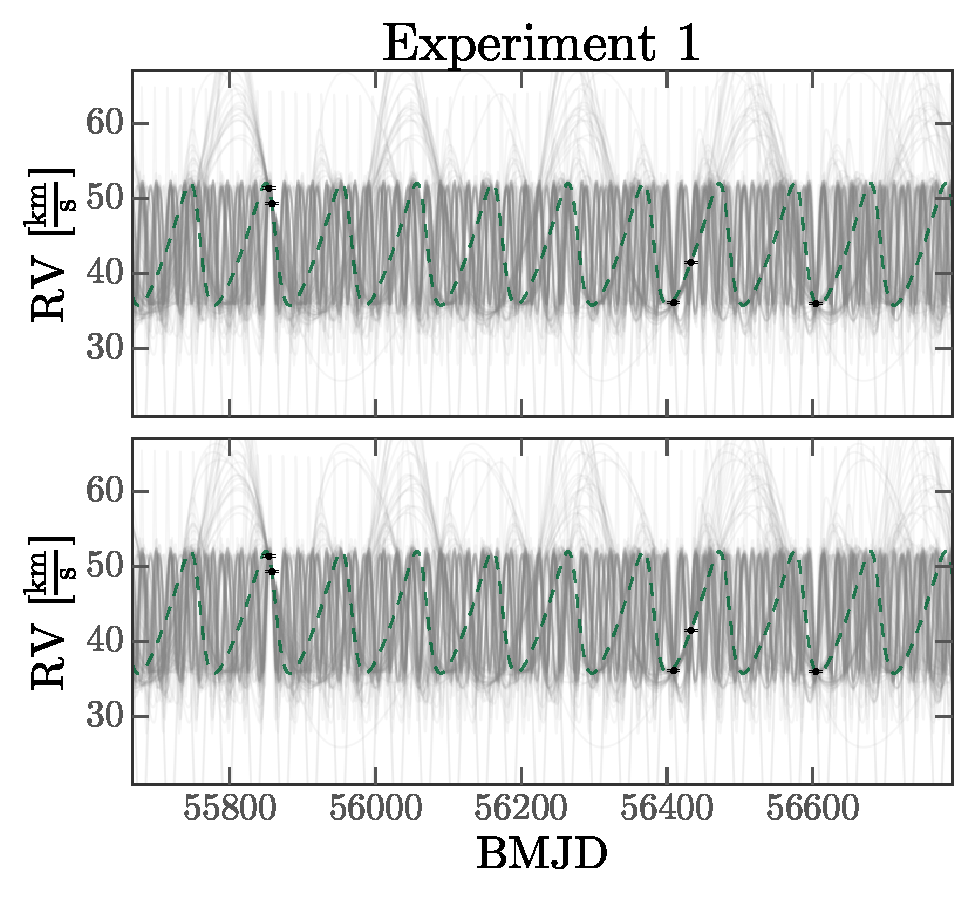
\includegraphics[width=\textwidth]{figures/exp1-rv-curves.pdf}
\end{center}
\caption{%
{\sl Top panel}: Black points show simulated radial velocity measurements
plotted against Barycentric Modified Julian Date (BMJD) of the observations.
Dashed green line shows the true, input orbit that the radial velocity
measurements were drawn from.
Grey curves show orbits computed from 128 samples from the posterior pdf for
these data.
Several qualitatively different orbital solutions are found over a range of
eccentricities and periods.
{\sl Bottom panels}: Projections of the posterior samples (grey points) and
value of true, input orbit (green +).
\label{fig:exp1-rv}}
\end{figure*}

\begin{figure*}[p]
\begin{center}
\includegraphics[width=\textwidth]{figures/exp1-corner.pdf}
\end{center}
\caption{%
All projections of the 30,082 surviving posterior samples (grey points) with
value of true, input orbit shown as green cross-hairs.
\label{fig:exp1-corner}}
\end{figure*}

\subsection{Experiment 2: A system known to be a binary with few observations}

For a more realistic application of \samplername, we choose an \apogee\ target
with a previously identified companion (2M00110648+6609349) but with few radial
velocity measurements (\citealt{Troup:2016}).
\figname~\ref{fig:exp2-rv}, top panel, shows radial velocity data for the star
(black points).\footnote{We don't plot the best-fit orbit from
\citealt{Troup:2016} because the parameter values reported in their work do not
produce Keplerian orbits that look like reasonable fits to the data.
\todo{APW: say this better / nicer?}}
Similar to Experiment 1, these data are sparse and have poor phase coverage,
however the time sampling is quite different and is representative of realistic
survey design choices.

We again generate $2^{28}$ prior samples over the nonlinear parameters with a
period domain of $(P_{\rm min}, P_{\rm max}) = (16, 8192)~{\rm day}$, of which
45,242 samples pass our rejection sampling step.
Over-plotted as grey lines on the top panel of \figname~\ref{fig:exp2-rv} are
128 orbits computed from random samples from the posterior pdf, sampled using
\samplername.
From these orbits, it appears that there are at least a few distinct period
modes, and a wide variety of eccentricities, represented in the posterior
sampling.
As with \figname~\ref{fig:exp1-rv}, bottom panels show two projections of the
posterior samples (grey points), but now the blue plus mark indicates the
previously found orbital parameter values (\citealt{Troup:2016}).

\figname~\ref{fig:exp2-corner} shows projections of all posterior samples in
different parameter combinations.
Here it is clear there are at least three period modes: the dominant mode at $P
\approx 300~{\rm day}$ is broadly consistent with the previously measured period
(\citealt{Troup:2016}), but other modes are clearly present at shorter periods
with low eccentricity and longer periods with higher eccentricity.

\begin{figure*}[p]
\begin{center}
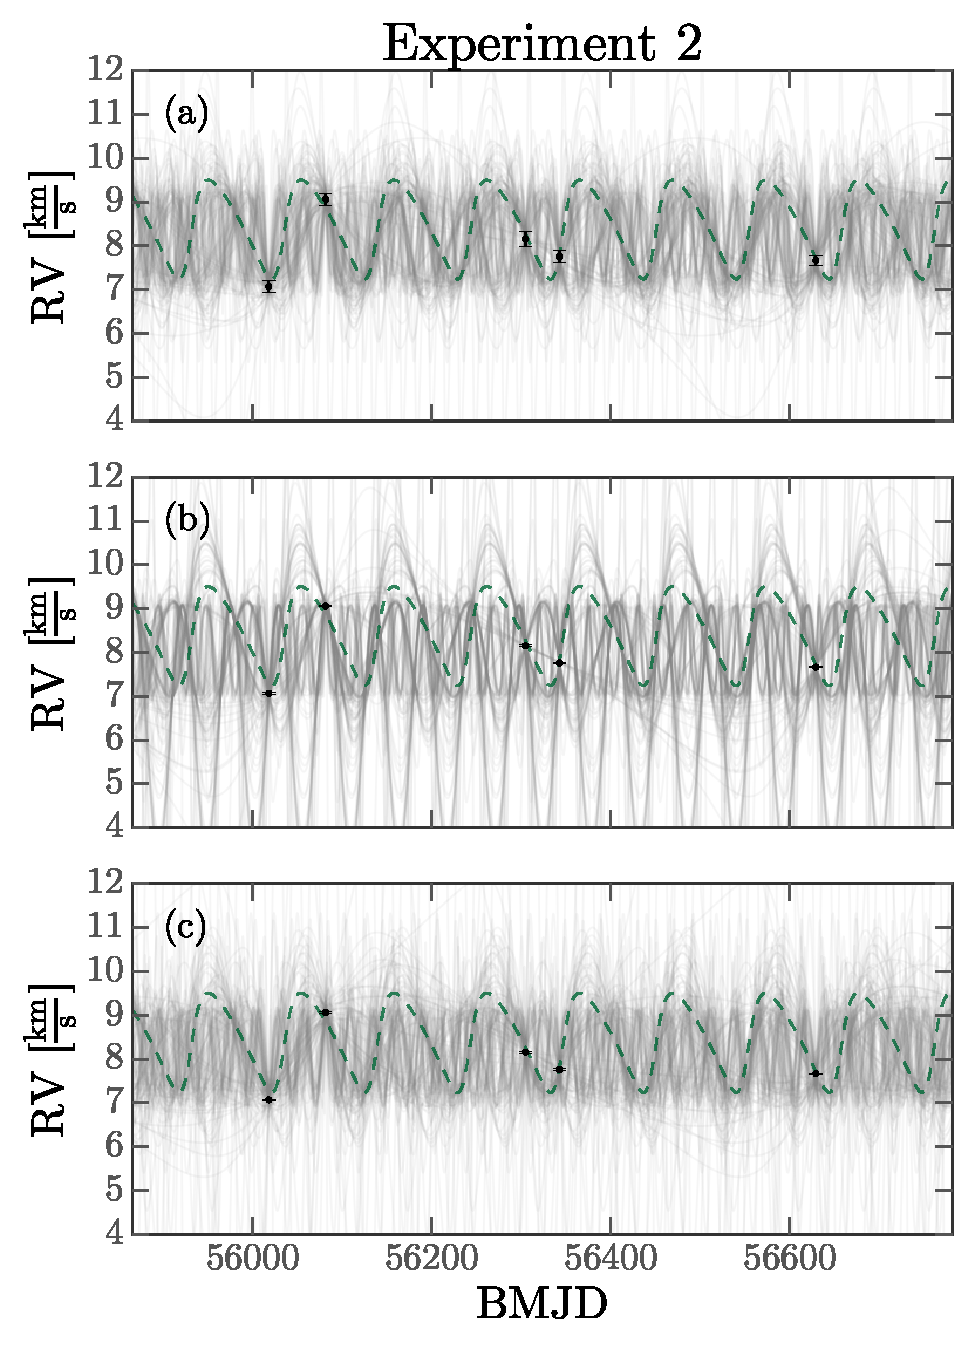
\includegraphics[width=\textwidth]{figures/exp2-rv-curves.pdf}
\end{center}
\caption{%
Same as \figname~\ref{fig:exp1-rv} but now using \apogee\ radial-velocity
measurements of the target 2M00110648+6609349.
Blue plus mark in bottom panels indicate orbital parameter values found in a
previous study (\citealt{Troup:2016}).
\label{fig:exp2-rv}}
\end{figure*}

\begin{figure*}[p]
\begin{center}
\includegraphics[width=\textwidth]{figures/exp2-corner.pdf}
\end{center}
\caption{%
All projections of the 45,242 surviving posterior samples (grey points) with
previously found orbital parameter values shown as the blue cross-hairs.
\label{fig:exp2-corner}}
\end{figure*}

\subsection{Experiment 3: Varying the number of data points}

When the phase coverage of the radial velocity observations is good and the
number of observations is large, the posterior pdf over orbital parameters will
likely be unimodal.
Under these conditions, \samplername\ is a very inefficient sampler for this
problem and will return very few samples (as few as one).
As we have seen in the previous experiments, when the number of data points
decreases, the posterior pdf will generally become more multi-modal.
He we study the dependence of the complexity of the posterior pdf on the number
of observations by using another \apogee\ target with a previously identified
companion (2M03080601+7950502) by successively and randomly removing
observations from the repeated analysis of these data with \samplername.
In DR13, this target has 30 visits; we remove 13 of these observations at random
so that we begin with 17 observtions.
After running the sampler with the set of 17 visits, we successively remove 2
data points and re-run the sampling until we are left with 3 observations as
input data (a total of 8 consecutive runs).

In detail, we again generate $2^{28}$ prior samples over the nonlinear
parameters with a period domain of $(P_{\rm min}, P_{\rm max}) = (16, 8192)~{\rm
day}$ and re-use these prior samples for each sub-sampling of the data.
\figname s~\ref{fig:exp3-rv-0}--\ref{fig:exp3-rv-1} show the data and orbits
computed from posterior samples returned by \samplername.
Starting from the top of \figname~\ref{fig:exp3-rv-0} with the full set of 17
measurements, each panel below has 2 fewer data points than the previous.
The data used for the sampling shown in a given panel are plotted as black
circles.
The number of measurements used, $N$, and the number of samples that survive the
rejection step, $M$, after one run of \samplername\ are indicated on each panel.
As described in \sectionname~\ref{sec:method}, when $M < M_{\rm min}=128$ we
either (1) if the periods of the surviving sample(s) are sufficiently close,
initialize \emcee\ using the remaining sample(s), or (2) re-run \samplername\
with a new set of prior samples until we have at least $M_{\rm min}$ samples
from the posterior pdf.
In all panels, 128 orbits computed from the posterior samples are shown.

For all sub-samplings shown in \figname~\ref{fig:exp3-rv-0}, the posterior pdf
appears to be uni-modal.
The structure in the posterior samples shown in the right panels of
\figname~\ref{fig:exp3-rv-1} is much more interesting.
Already in the top panels ($N=9$), multiple modes appear.
These become more apparent in the panels below, until ultimately forming a
harmonic series of modes in the bottom two rows of panels.
This highlights the highly complex but structured posterior pdfs that are
expected for stars with very few radial velocity measurements.
Still, we are able to sample from these pdfs using \samplername.

\begin{figure*}[p]
\begin{center}
\includegraphics[width=\textwidth]{figures/exp3-rv-curves-0.pdf}
\end{center}
\caption{%
{\sl Left panels}: Similar to top panel of \figname~\ref{fig:exp1-rv}, black
points show \apogee\ radial velocity measurements used to generate samples from
the posterior pdf over orbital parameters sub-sampled from the full set of
observations for this target 2M19405532+2401157.
Grey curves show orbits compute from 128 samples from the posterior pdf, either
from using \samplername, or, if \samplername\ returns few samples in a small
range, from switching to \emcee\ to continue sampling until 128 samples are
returned.
The number of data points, $N$, and the number of samples that pass the
rejection sampling in the first step of \samplername, $M$, are printed on each
panel.
{\sl Right panels}: A single projection of the posterior samples in each case
showing the log-period, $\ln P$, and eccentricity, $e$.
In all cases shown, the posterior pdf appears to be uni-modal.
\label{fig:exp3-rv-0}}
\end{figure*}

\begin{figure*}[p]
\begin{center}
\includegraphics[width=\textwidth]{figures/exp3-rv-curves-1.pdf}
\end{center}
\caption{%
Same as \figname~\ref{fig:exp3-rv-0} for further sub-samplings of the original
data set.
Note that the axis limits for the right panels have expanded considerably, and
that there are multiple modes in the posterior pdf for all cases in this figure.
\label{fig:exp3-rv-1}}
\end{figure*}

% \figname s~\ref{fig:exp3-corner-0}--\ref{fig:exp3-corner-1} show a few
% projections of the posterior samples for each of the data sub-samplings (i.e.
% the panels in these figures match the panels in
% \figname s~\ref{fig:exp3-rv-0}--\ref{fig:exp3-rv-1}).
% All panels in \figname s~\ref{fig:exp3-corner-0} show that the posterior pdf is
% very compact and unimodal when $N=19,17,15,13$ data points are used.
% We have fixed the axis limits to be the same in \figname
% s~\ref{fig:exp3-corner-0} and \ref{fig:exp3-corner-1}), so the single dark point
% in some of the panels of \figname~\ref{fig:exp3-corner-0} are very compact
% visualizations of the posterior samples.

% \begin{figure*}[p]
% \begin{center}
% \includegraphics[height=0.9\textheight]{figures/exp3-corner-0.pdf}
% \end{center}
% \caption{%
% TODO
% \todoapw{More comments here..}
% \label{fig:exp3-corner-0}}
% \end{figure*}

% \begin{figure*}[p]
% \begin{center}
% \includegraphics[height=0.9\textheight]{figures/exp3-corner-1.pdf}
% \end{center}
% \caption{%
% Same as \figname~\ref{fig:exp3-corner-0} for smaller sub-samplings of the
% original data set.
% \todoapw{More comments here..}
% \label{fig:exp3-corner-1}}
% \end{figure*}

\subsection{Experiment 4: Increasing the uncertainties}

Another aspect of the data that determines the complexity of the posterior pdf
are the uncertainties on the individual data points.
To explore this, we again use the \apogee\ target 2M03080601+7950502 and
downsample the data points so that there are 17 observations (the same as shown
in the top panels of \figname~\ref{fig:exp3-rv-0}).
We then steadily increase the uncertainties on the individual radial velocity
measurements by factors of 2 and run \samplername\ to generate posterior
samples.
We again generate $2^{28}$ prior samples over the nonlinear parameters with a
period domain of $(P_{\rm min}, P_{\rm max}) = (16, 8192)~{\rm day}$ and re-use
these prior samples for each iteration of increasing the uncertainties.

\figname~\ref{fig:exp4-rv} shows the data and uncertainties (left panels, black
points), 128 orbits chosen at random from the posterior sampling, and all
samples plotted in projection of log-period, $\ln P$, and eccentricity, $e$.
The data in the top panel of \figname~\ref{fig:exp4-rv} have uncertainties
artificially increased by a factor of 2 relative to the data in the top panel of
\figname~\ref{fig:exp3-rv-0}, and each successive row has another increase by a
factor of 2.
For this particular target, increasing the uncertainties by a factor of 4 or
more makes the posterior pdf multi-modal, even with 17 observations over a range
of phases.

\begin{figure*}[p]
\begin{center}
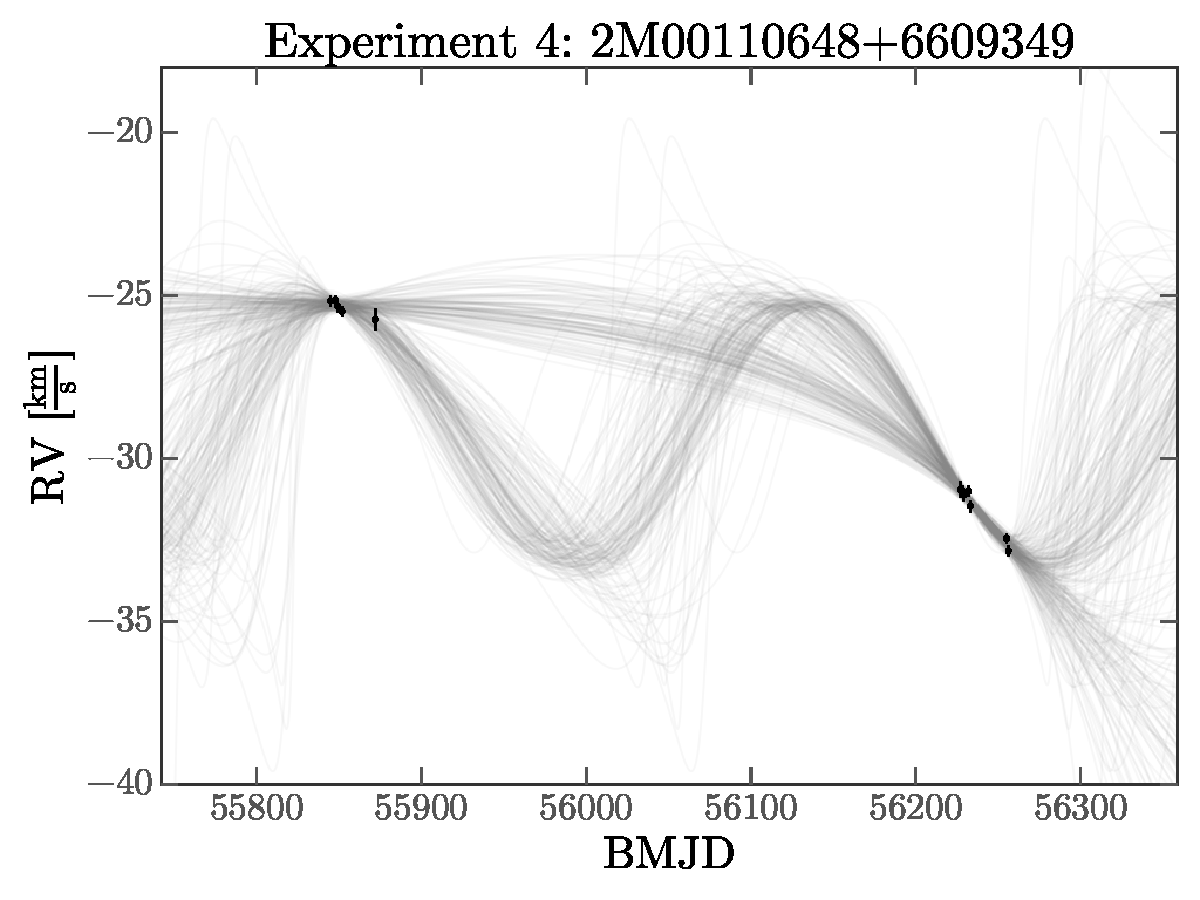
\includegraphics[width=\textwidth]{figures/exp4-rv-curves.pdf}
\end{center}
\caption{%
Similar to \figname~\ref{fig:exp3-rv-0} but now varying the magnitude of the
uncertainties instead of the number of data points.
Each row has uncertainties increased by a factor of 2 relative to the previous
row.
The mean value of the uncertainties for all data points is shown on the left
panels as $\langle \sigma_n \rangle$, along with the number of samples that
survive the rejection sampling with \samplername\, $M$.
\label{fig:exp4-rv}}
\end{figure*}

\subsection{Experiment 5: Prospects for observation planning}

A noticable feature of the middle two panels of \figname~\ref{fig:exp3-rv-1} is
that the posterior pdf collapses significantly between the $N=5$ and $N=7$
cases.
This implies that the two added observations are extremely informative, and that
we can use \samplername\ to predict when observations would be most valuable for
a given source.
We will explore this topic in detail in future work, but here we simply show
that the timing of subsequent observations can lead to very different
structure in the posterior samples.

We again simulate a data set of four noisy radial velocity measurements, shown
as black points in the top-left panel of \figname~\ref{fig:exp5-rv}.
Uncertainties were chosen to match the \apogee\ data ($\sigma_v \approx
0.2~\kms$) and are shown as error bars, but they are often comparable to or
smaller than the marker size.
Top-right panel shows posterior samples produced with \samplername\ again in the
space of log-period $\ln P$ and eccentricity $e$.
The three lower rows all have six observations: the same four from the top row,
but now with two additional observations spaced, in phase, by $\frac{\Delta
\phi}{2 \pi} = 0.04$ but with a different starting phase for the new
observations.
As is shown by the right panels, the observation times of the new observations
can greatly effect the compactness of the posterior pdf.
In particular, the placement of the observations in the bottom row of panels
rules out most of the long-period modes from the top panels, \emph{and} many of
the short-period modes, whereas for the middle two cases the new data are not as
informative.

\todo{Add N, M to the panels to show the number of data points and the number of
surviving samples!}
\todo{Add another panel to the figure with the subsequent two observations at a
bad postion (doesn't collapse pdf)}

\begin{figure*}[p]
\begin{center}
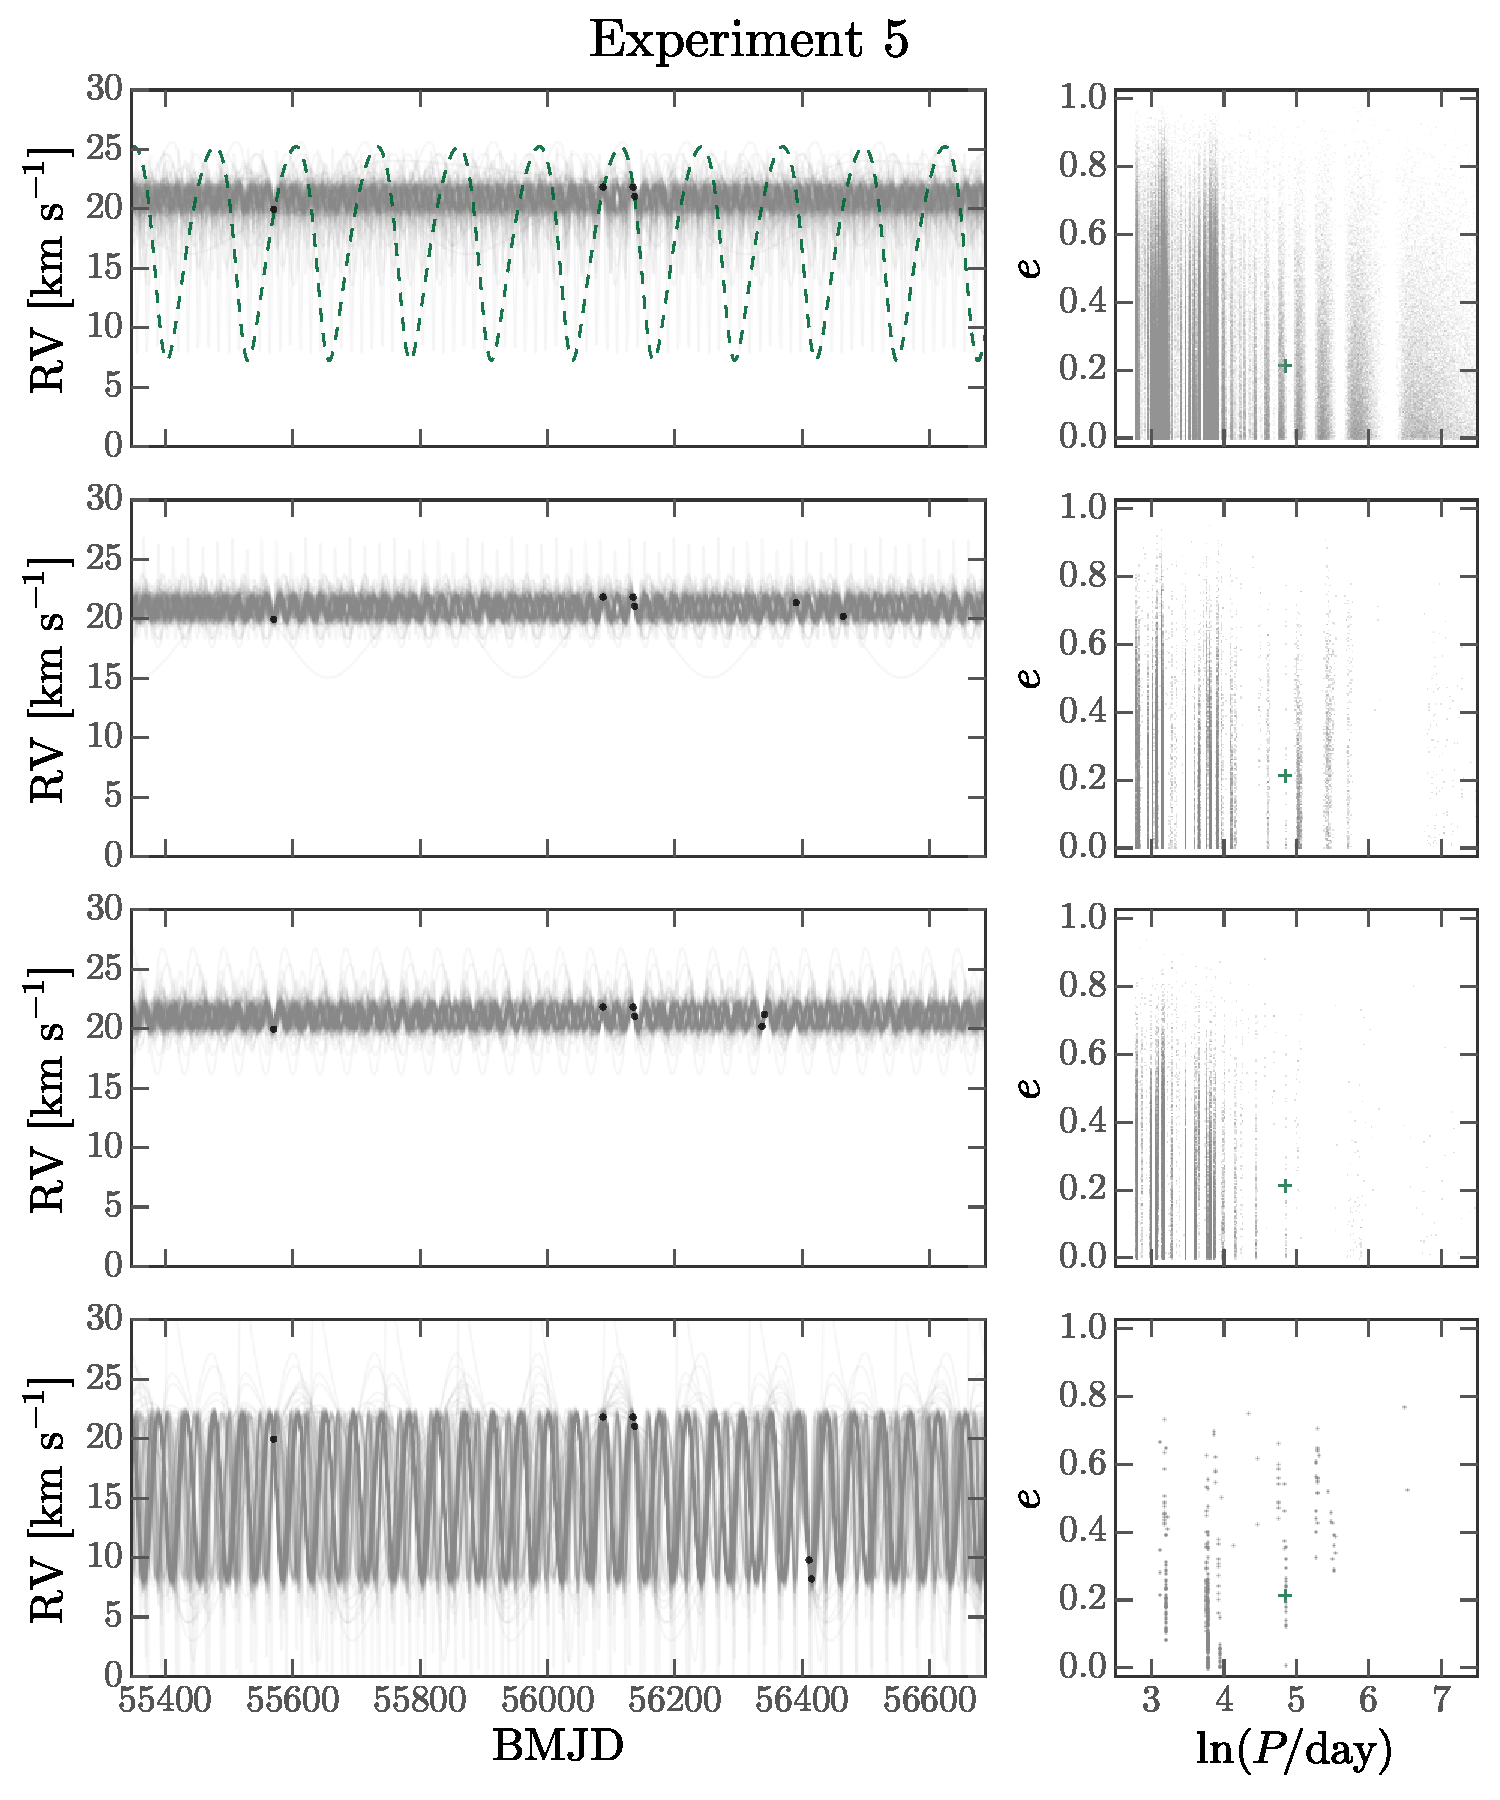
\includegraphics[width=\textwidth]{figures/exp5-rv-curves.pdf}
\end{center}
\caption{%
\todo{Draw the truth RV curve on the top panel}
Similar to \figname~\ref{fig:exp3-rv-0} and \figname~\ref{fig:exp4-rv} but now
varying the timing of new simulated observations relative to the data in the
top-left panel.
The top row has four simulated observations and all of the rows below the top
row have two additional observations placed at different times but with fixed
spacing in phase; the number of data points $N$ and number of samples that
survive the rejection sampling $M$ are shown on each panel.
\label{fig:exp5-rv}}
\end{figure*}

\section{Discussion} \label{sec:discussion}

We have built a Monte Carlo sampler---\samplername---for the
single-companion radial-velocity problem that has very good
properties:
It produces fair samplings even when the likelihood (and hence
posterior pdf) is highly multi-modal.
The cost of this fair sampling is computer time:
Our method is based on Simple Monte Carlo, which is a pure brute-force
method.
The primary innovation we bring is a separation of the parameters
into linear and nonlinear subsets, such that the brute force is only
required in the nonlinear subspace.
We further capitalize on the problem structure by identifying unimodal
and multi-modal posterior pdfs using the minimum possible width of a
likelihood peak in the period direction, given the time sampling.

Our experiments show that \samplername\ can be used for discovery and
characterization of stellar binaries or exoplanets.
It can also be used to generate inputs for a hierarchical inference.
In previous work (\citealt{hoggeccentricity, dfmexopop}) we have shown
that posterior samplings under an interim prior can be importance-sampled
with a hierarchical inference to generate posterior beliefs about the
full population.
These---hierarchical inferences---are the only population inferences
that properly propagate non-trivial uncertainties at the
individual-system level to the conclusions at the population level.

Interestingly, as we show in Experiment~APW:WHAT, even very sparse
samplings of the radial-velocity history of a star provide highly
informative posterior pdfs.
Panel APW:WHAT in \figurename~APW:WHAT shows a highly multi-modal
posterior pdf, but nonetheless a very informative posterior pdf:
The vast majority of prior pdf samples have been eliminated, and
only a tiny subset of periods, eccentricities, and amplitudes are
consistent with the data.
These posterior pdfs may look like a mess, but they would contribute
extremely valuable information to any hierarchical inference, or
provide a very informative prior pdf for further observing campaigns.

Indeed, one of the purposes for which we built \samplername\ is
observation planning, or cadence evaluation, or survey strategy:
As Experiment~APW:WHAT shows, \samplername\ could be used to plan the
times of next observations to maximize their expected information
content.
That is beyond the scope of this \documentname, but it is not beyond
the scope of our ambitions.

\samplername\ is based on a set of assumptions, itemized in
\sectionname~\ref{sec:method}; indeed, the method delivers provably
correct samplings when these specific assumptions hold.
Of course, these specific assumptions do \emph{not} hold!
There is never any guarantee that a star's radial-velocity history
is set entirely by a single companion, with no other perturbers or
sources of radial-velocity signal.
More importantly, there are no data sets (to our knowledge) with
perfectly Gaussian noise, and even if there were, the noise variances
could never be perfectly known!

Although the single-companion assumption is a severe assumption, it
is pretty-much required for the method to be tractable.
Of course, in reality, it is likely that most stars have thousands or
millions of companions (the Sun does, after all).
Even going to two companions, however, the non-linear parameter space
jumps to eight-dimensional, and (at least) ten-dimensional if there
are companion--companion interactions.
This would be absolutely intractable to sample by brute-force Simple
Monte Carlo; our advice would be to switch to some kind of Markov
Chain method that deals as well as possible with multi-modal
posteriors, such as nested sampling (\citealt{skilling, brewer}).
This change would be associated with the loss of the simple
convergence criterion that Simple Monte Carlo provides: If lots of
samples survive the rejection step, the posterior has been sampled
fairly!
There is no comparably simple way of determining that any nested
sampling is converged.

That said, there is a simple three-body problem that \emph{can} be
solved tractably, with only small modifications:
If the third body is on a very long-period orbit, it appears only
as an overall acceleration (velocity gradient with time).
This can be modeled with just one more parameter, and that parameter
is linear, so it doesn't worsen the prior pdf sampling (which happens
over the nonlinear parameters only).

Actually, the number of linear parameters could be increased
dramatically without any serious loss of performance, since almost all
of the compute time is taken up with the dense sampling in the nonlinear
subspace.
These extra linear parameters could be the extra $v_0$ terms that come
in when, say, the data come from a set of different radial-velocity
programs with different calibrations (as is the case for the recent,
impressive Proxima b discovery; \citealt{proximab}).
Another case for additional linear parameters would be the regressing
out of confounding signals that correlate with housekeeping data,
like, say, radial-velocity shifts that correlate with activity signals
(HOGG CITE?).

Although we have argued that our prior pdf sampling is dense enough,
and---by God---we spend enough time on it, it might not be dense enough
if we push to very short periods.
The problem structure points (in \sectionname~\ref{sec:method})
includes the point that, given a finite time span for the data, there
is a finite width to any period peak in the likelihood function.
This finite width goes like period squared, so at very short periods,
it gets very narrow.
Our prior sampling is uniform in the logarithm of period, or the
density of samples in period goes like inverse period.
If we wanted to make sure a minimal prior sampling was always dense
enough at every period, we should weight it by an additional factor of
inverse period.
A change like this could improve the reliability of the method when the data
are informative, the observations span a long time, and the true
period is short.
For now \samplername\ simply addresses the prior sampling density issues
by using as many prior samples as it possibly can!

All these caveats noted, \emph{by far} the worst assumption made by
\samplername\ is that the noise is Gaussian with known variances:
All data sets show occasional outliers (catastrophic errors), almost
all data sets under-estimate the true radial-velocity errors, and the
fact that the radial-velocity measurments depend on stellar parameters
(the stellar photosphere model, say) leads to added radial-velocity
noise, usually unaccounted for.
What can we do in these cases?
There is nothing we can simply do here, if we want to maintain the
trick of treating the linear and non-linear parameters separately.
Our advice to users who believe that they have additional sources or
forms of noise is to inflate the uncertainty variance estimates and
try to get conservative conclusions about the posterior pdf.

If the only problem is an underestimate of the noise variances, the
factor or offset to be applied to the variances can be promoted to a
non-linear parameter and sampled along with the other nonlinear parameters.
This is probably (just) practical.
If the only problem is occasional outliers, the method could be
modified to do all leave-one-out samplings, take the union, and then
importance sample the results using some ratio of the mixture of
leave-one-out Gaussian likelihoods to some more realistic likelihood
that involves an outlier model (as, for example, we suggest in
\cite{fittingalline}).
These modifications to the method are beyond the scope of this
\documentname\, but (once again) not beyond the scope of our ambitions.

\acknowledgements
This project was started at AstroHackWeek 2016, organized by Kyle
Barbary (UCB) and Phil Marshall (SLAC) at the Berkeley Institute for
Data Science.
It is a pleasure to thank
  Megan Bedell (Chicago),
  Ben Weaver (NOAO),
  and the participants at AstroHackWeek 2016
for valuable discussions.

This research was partially supported by
  the \acronym{NSF} (grants \acronym{IIS-1124794}, \acronym{AST-1312863}, \acronym{AST-1517237}),
  \acronym{NASA} (grant \acronym{NNX12AI50G}),
  and the Moore-Sloan Data Science Environment at \acronym{NYU}.
The data analysis presented in this article was partially performed on
computational resources supported by the Princeton Institute for Computational
Science and Engineering (PICSciE) and the Office of Information Technology's
High Performance Computing Center and Visualization Laboratory at Princeton
University.
This work additionally used the Extreme Science and Engineering Discovery
Environment \citep[XSEDE;][]{Towns:2014}, which is supported by National
Science Foundation grant number ACI-1053575.

This project made use of \sdssiii\ data. Funding for \sdssiii\ has been
provided by the Alfred P. Sloan Foundation, the Participating Institutions, the
National Science Foundation, and the \acronym{U.S.} Department of Energy Office
of Science. The \sdssiii\ web site is \url{http://www.sdss3.org/}.

\sdssiii\ is managed by the Astrophysical Research Consortium for the
Participating Institutions of the \sdssiii\ Collaboration including the
University of Arizona, the Brazilian Participation Group, Brookhaven National
Laboratory, Carnegie Mellon University, University of Florida, the French
Participation Group, the German Participation Group, Harvard University, the
Instituto de Astrofisica de Canarias, the Michigan State/Notre
Dame/\acronym{JINA} Participation Group, Johns Hopkins University, Lawrence
Berkeley National Laboratory, Max Planck Institute for Astrophysics, Max Planck
Institute for Extraterrestrial Physics, New Mexico State University, New York
University, Ohio State University, Pennsylvania State University, University of
Portsmouth, Princeton University, the Spanish Participation Group, University
of Tokyo, University of Utah, Vanderbilt University, University of Virginia,
University of Washington, and Yale University.

\software{The code used in this project is available from
\url{https://github.com/adrn/thejoker} under the MIT open-source software
license. This version was generated at git commit
\texttt{\githash\,(\gitdate)}.
This research additionally utilized:
    \texttt{Astropy} (\citealt{Astropy-Collaboration:2013}),
    \texttt{emcee} (\citealt{Foreman-Mackey:2013}),
    \texttt{IPython} (\citealt{Perez:2007}),
    \texttt{matplotlib} (\citealt{Hunter:2007}),
    and \texttt{numpy} (\citealt{Van-der-Walt:2011}).}

\facility{\sdssiii, \apogee}

\bibliographystyle{aasjournal}
\bibliography{thejoker}

\end{document}
